% Chapter Template

\chapter{Conclusion} % Main chapter title

\label{Conclusion} % Change X to a consecutive number; for referencing this chapter elsewhere, use \ref{ChapterX}

%----------------------------------------------------------------------------------------
%	SECTION 1
%----------------------------------------------------------------------------------------
\section{Project Status and Possible Improvements}
 
The current project is working and has reached all the objectives mentioned in the requirement specifications. Nonetheless, there is plenty of room for improvement. The current architecture could itself profit of some optimization but this design itself could be restructured to greatly improve its performance. Indeed, the current model suffers from huge memory induces delays, more than 90\% of the execution time is actually spent waiting for HMC data.\\

This section will first discuss the current architecture and what small changes could improve its performances. Then, it will propose two architectures derived from the current one that would be far more performant. Finally, others aspects of the project will be discussed.

\subsection{Current Architecture}

The current architecture suffers from two major performance faults :
\begin{enumerate}
    \item For every request made to the HMC, the interface waits for its response. Thus restricting to one the number of request that can be made in parallel.
    \item The HMC interface does not keep any data locally, hence, two consecutive request for the same data will result in two full request made to the memory with no data reuse whatsoever.
    \item Although the full \textit{bounds} interval is computed, only the first position is used to get the position in the original text.
\end{enumerate}

For each of these flaws, a simple fix could be introduced that would greatly restrict their impact on performance, respectively :

\begin{enumerate}
    \item The HMC Interface could use the \texttt{tag} parameter when sending request to the HMC in order to send multiple request consecutively while being able to keep track of the response. This would not only allow several blocks to make request at the same time, but also the same block to issue several consecutive requests (e.g. Last-First in its iteration phase) and wait only once the big response delay. Of course, two process' would be needed in the interface, in order to be able to process request and responses at the same time.
    \item By simply keeping track of the most recent requests, the HMC Interface could spare a lot of requests, especially during the iterative loop of the Last-First Mapping algorithm. Indeed, during this asks for consecutive symbols of the BWT. At the moment, even though the data requested to the HMC is the same, the interface makes a new requests and waits for the response. A simple buffer based specifically on this request would on average reduce the time required for this mapping at least 10-fold.
    \item With a simple modification of Walk-Left's FSM, it would be easy to consecutively \textit{walk back} for a limited number of positions contained in the provided interval and keep the results in a local buffer. Those could then be sent back consecutively through the stream with little modifications in the software.
\end{enumerate}

\subsection{Proposed Architectures}

A first and most intuitive idea would be to duplicate the whole FM-Index bloc. Moreover, there are 5 independent HMC ports available to communicate with the HMC, thus, all could be used and assigned to a certain number of FM-Index blocs. Figure \ref{fig:FM_DUPL} shows how \textit{reds\_top} could be adapted to process multiple short reads in parallel. \\
The parameters such as the Occ array and the BWT size are shared among all the instances of the FM-Index. The short reads are place in a FIFO, accessible from all instances, of course this FIFO would need to be of a fixed width and depth, that would limit said reads size to under a pre-defined constant. \\
Every memory request from a FM-Index instance is placed into a FIFO, shared with several others instances. The index of each instance is used as a tag to place the memory response at the right buffer offset. \\
Finally, every instance, once done processing their current data, places their result into a FIFO feeding the output stream. 

\begin{figure}[H]
    \centering
    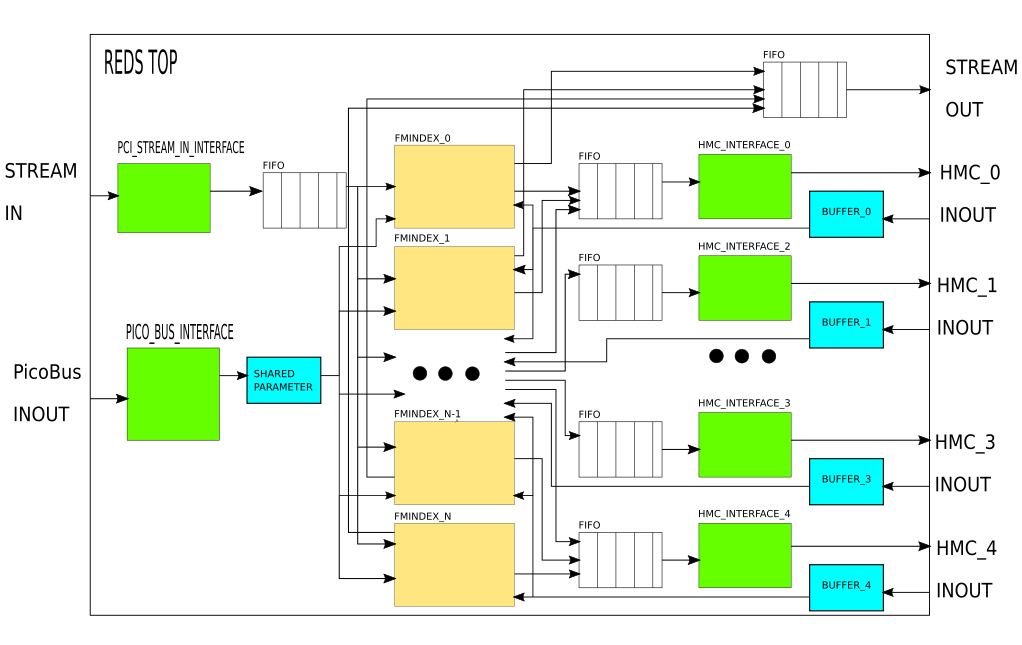
\includegraphics [scale = 0.4]{Figures/FMINDEX_DUPL_DIAG.png}
    \caption{Gross Bloc Diagram of duplicate FM-Index Bloc in Reds\_Top}
    \label{fig:FM_DUPL}
\end{figure}

This architecture, although it enables some degree of parallelization, still presents some major flaws. A first and most prohiminent one would be that each instance of the FM-Index is still only issuing one request at a time, thus still very slowed by the stall between all memory request. \\


Another and more efficient idea would be to enable parallelism inside the FM-Index. In order to do so, the FSM must be broken down into a set of independent transactions. \\
As long as there are central memory blocs to keep tracks of a short read ID and processing state (top and bot value, walk back value, current row, etc.). By using memory blocs to keep track of those values, and FIFO to feed the different blocks, the sequential FSM could be transformed into a finely pipelined process. Figure \ref{fig:FM_FIFO} depicts a gross representation of what could such an architecture look like. \\

The main advantage of this architecture, despite being much more complex - and thus much harder to test and validate, is that this whole block could itself be duplicated in the \textit{reds\_top} layer. \\

This architecture would seem to be the most efficient both space-wise ine the FPGA, and time-wise by minimizing the stalling time between HMC requests and responses. On the other hand, the overhead induced by the synchronization and coordination of those transactions would then not be negligible.

\begin{figure}[H]
    \centering
    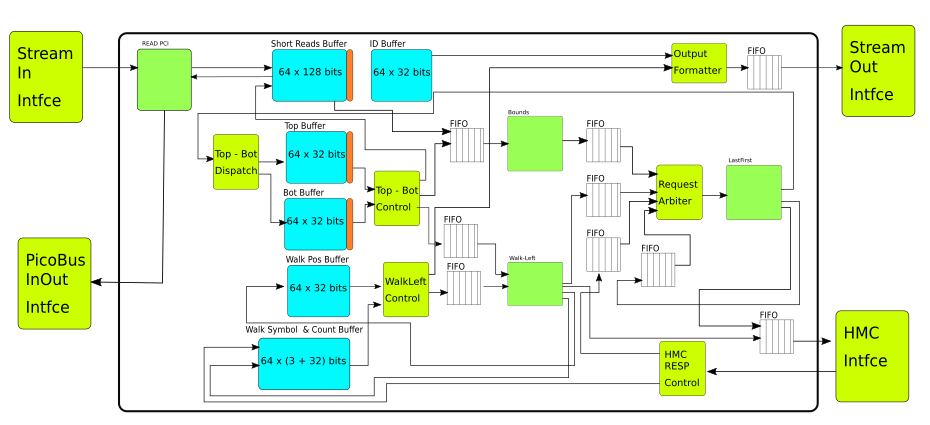
\includegraphics [scale = 0.5]{Figures/FM_OPTI.png}
    \caption{Gross Bloc Diagram of an Optimized FM-Index}
    \label{fig:FM_FIFO}
\end{figure}

This architecture would be able to process 64 short reads in parallel, chunk by chunk (fixed by the width of the buffer). The modification are further explained in the paragraph below.
Roughly, the idea would be the following :
\begin{description}
    \item [Short Read Buffer] - This buffer contains fixed size chunks of provided short reads, the orange column corresponds to a bit indicating whether the line is done or not, i.e. whether ReadPCI should notify the software to send another chunk for a specific short read through the PicoBus.
    \item [Top, Bot Buffer - Bounds] Two buffers that are kept in sync with one another and with their corresponding short read by the \texttt{Top-Bot Control} and \texttt{Top-Bot Dispatch} blocks. The first would evaluate whether the Bounds processing is finished and whether both Top and Bot have been computed for the current symbol. If that's the case, it shifts the corresponding short read and proceed with the next step. The latter is used to dispatch Last-First response to the correct buffer and update the flag column with the current iteration index.
    \item [Last-First] This bloc would be the most demanded by the system, hence the breakdown of its internal loop seemed necessary, along with an arbiter for its input requests. The loop in which LF iteratively reads the BWT, until reaching a checkpoint entry, would be separated from the direct checkpoint request, hence the different buffers. This block can then receive data from Bounds for a position update, Walk-Left for a BWT symbol, the HMC for a response and from itself during the iterative loop.
\end{description}

The remaining elements speaks for themselves and will not be discussed. Now despite the estimated efficiency of this architecture, its complexity and entanglement between the different phases of the algorithm would make it way harder to observe and debug, which is the main issue in hardware design.

\subsection{Global Possible Improvements}

In their current state, the testbenchs don't seem thorough enough. Those limit indeed their verification to the correctness of the data, with little to no consideration for timing. Furthermore, implementing a serie of addressed registers that would be reachable from the software and provide information about the system parameters or current states would be more than welcome. Currently, it is only possible to write parameters at the beginning of the execution (such a the transform size and the occ array). Adding an interface that would enable reading pertinent information about the system would not require a lot of modification of the system itself, while greatly improving the comfort of the developpment phase. \\


On the software side, the current version could be improved by offering a better output formatting and a less restrictive input interface. Indeed, it would be more comfortable to be able to interact with the program while waiting for a result (e.g. probe the hardware system, load other files, etc.).


\section{Personal Comment}

Globally, this project in its current states remains unfinished. Most of the late efforts where not aiming to an optimal solution but a functioning one and an additional week or two of work would have make a difference. Not only in the tidiness of the code, but also on the global optimization that could be done. \\

It seemed necessary to go through a rather crude implementation before being able to grasp to complexity of the system and being able to optimize its operation and interactions with the memory. Integrating the FM-Index into the whole PicoProject required days of work in order to understand the interaction between the different entities but to understand and correct a global behavior that was not anticipated, such as the activity on the different I/O bus'. Thus, this step should have happened a lot earlier than it did, and maybe more could have been concretely done. Instead, a lot of theoretical models for optimized architecture were made, in vain since it took all the remaining time to make the more basic one work on the board. \\

In conclusion, one could say that, surprisingly, several predictable but unforeseen delays have been induced by a bad estimation of the complexity of the system to implement, and the platform it has been made for. Nonetheless, the resulting system is fully functional and offers a great baseline for future improvement, thus despite leaving a tiny bitter taste of unfulfilled ambitions, this project remains a very satisfactory result.

\section{Acknowledgment}

This thesis has been by far the most complex and interesting project I've had the opportunity to work on. I would like to thanks Prof.Thoma for his guidance and his advice full of wisdom during the whole project. I would also like to thank M.Wertenbroeck who offered me help and counseling from the beginning and until the end. \\

Furthermore, I would like to thank [TODO]\\

And to conclude on a pragmatic note and a yet relevant opinion about this career area and the glance at a bright future in this domain this Bachelor brought to me, I would like to share a quote from an eminent member of the Computer Science community.


\epigraph{"I used to think that everybody should learn programming. When I first started learning –thinking about how to organize the world in terms of data structures and algorithms– I thought, "Wow, this is such an amazing way to organize information. Everybody should learn to do this!" \\

I don't think that anymore. \\

I think there has to be something seriously wrong with you in order to do this work. A normal person, once they’ve looked into the abyss, will say, “I’m done.[...] I’m going to do something else.” But not us, because there’s something deeply wrong with us."}{\textit{Douglas Crockford, Senior JavaScript Architect}}